\section{Introduction}
We will discuss the terminology and technology used in this chapter in our project. We would also look at past work, strengths and limitations in this field. We also study the hardware parts used in this project.
\section{Related Literature Review}
~\cite{cloete2016design}
In ~\cite{gubbi2013internet} Gubbi et al., proposed a framework that has scalable cloud and capacity for the internet of things. They discussed IoT, ubiquitous computing and wireless sensor network. They showed how various sensors can be connected using a gateway to a cloud with the internet and work together. Cloud has services like analytic and visualization and the security of data. They discussed that computing devices like a computer can be connected to the public cloud-like Microsoft Azure, Amazon AWS, Google and iCloud. This all things can work together using the internet of things technology. This research paper tried to explain the overall architecture of the internet of things.
In ~\cite{geetha2016internet} Geetha et al., proposed a low-cost simple system based on the internet of things concept where they used pH sensor, turbidity sensor, conductivity sensor and a level sensor for getting the quality data of water. They used TI CC3200, a controller with a built-in wiFi module. After collecting data, they send those to a cloud server with the internet. And retrieve those data with the mobile device. They used a message sending system from the cloud to the users mobile when the value exceeds the predefined threshold.
In ~\cite{dong2015survey} Jianhua dong et al., discussed their survey on various water quality monitoring system till 2014. After the survey, they divided all the system into three subsystem data collection subsystem, data
transmission subsystem, and data management subsystem. In the data collection, part data is collected from various sensors like pH, conductivity, turbidity, residual chlorine etc., in the transmission, part data is transferred to the remote cloud using 3G, GPRS, microwave, GSM and satellite. In the management, part data is analysed, based on threshold cloud makes early warning.
In ~\cite{banna2014online} Banna et al., discussed in their research paper various chemical parameter for drinking water. They marked that the use of a sensor array for monitoring water quality at distributed system is costly. So they searched for better technology and focused on sensor technology.
%In ~\cite{barabde2015real}
In the research paper, ~\cite{lambrou2012low} Lambrou et al., proposed a system based on IoT technology where they focused on low cost, lightweight and reliability. They used analogue to digital converter for converting sensors data. Using Zigbee module data sent to the server and using router those data are received.
In research paper~\cite{kageyama2016wireless} Kageyama et al. proposed a dynamic floating system for monitoring water quality. In this system, a solar panel is the main power source and a battery for backup. After receiving data, it sends to the server using the GSM module which uses 3g technology. 
In ~\cite{hur2008using} Hur et al., developed a monitoring tool for predicting biochemical oxygen demand (BOD) using synchronous fluorescence technique. They found that protein-like fluorescence intensities of the water samples show a positive linear relationship with the BOD values.
In paper ~\cite{silva2011web} Silva et al., web-based wireless sensor network application that collects various water quality parameter and send those data through the Zigbee gateway to a web server using WiMax network and users can see the real-time water quality.
In ~\cite{priya2018design} Kavi Priya et al., proposed a low-cost system based on IoT technology for monitoring drinking water quality at the distribution system. The sensors are placed in the pipe through which the water passes. If the contamination occurs the Zigbee module sends signals to the solenoid to turn off the water supply and intimates the consumers about drinking water quality through a mobile app.
In ~\cite{prasad2015smart} Prasad et al., designed a system using IoT and remote sensing technology for Fiji. Where they collected sensors data and stored it in local storage and sent it to the cloud using GSM technology. The remote computer can download those data to see. 
In research paper~\cite{zhang2010design} Zhang et al. proposed a framework where they used IoT and wireless sensor network. The sensor network is the interconnection of many sensors. They used the Zigbee module to send data in the low range of distance and the GSM 3g network to send data to a long-range distance server. A database was to hold all data. By calculating those data if they found contamination then used early alarm system using GSM to notify users.

In ~\cite{cloete2016design} Cloete et al., proposed a system in which temperature, turbidity, pH, dissolved oxygen and
conductivity is measured and sent to a remote monitoring centre using Zigbee and CDMA (code
division multiple access) technologies. And when the quality is under the accepted level then a
buzzer makes an alarm. Which is not accessible globally Again there is no flow measurement.
In ~\cite{gopavanitha2017low} Gopavanitha et al., designed a system where the Temperature, Turbidity, Conductivity, pH and Flow of water is measured. By these sensors, water contaminants are detected. The sensor values processed by Raspberry pi and
send to the cloud. In this system, there is no alarm when the quality is going under the accepted level. And no measurement of how much water is used.
In ~\cite{de2017water} De Belen et al., proposed a system where the temperature, flow rate, and pH of water is measured. And a relation between temperature and pH is found. 
But this system has not any measurement of the volume of water, amount of used water, alarm system and does not send data to the cloud.
In ~\cite{raju2017knowledge} Raju et al., proposed a system where dissolved oxygen, ammonia, pH, temperature, salt, nitrates, carbonates are measured but no other features.
In ~\cite{lambrou2012low} Lambrou et al., proposed a system where turbidity, pH, the temperature is measured and sends those data to the local remote centre. Not directly to global server or cloud. And this system has not another feature.
In ~\cite{ramos2008four} Ramos et al., proposed this system where only electricity conductivity through water and temperature of can be measured. 
In paper ~\cite{vijayakumar2015real} Vijayakumar et al., said that the parameters such as temperature, pH, turbidity, conductivity, dissolved oxygen of the water can be measured. The measured values from the sensors can be processed by the core controller. The raspberry PI B+ model can be used as a core controller. Finally, the sensor data can be viewed on the internet using cloud computing. Multi-parametric sensors are thoroughly tested for water quality and pH values. But this system has no measurement of water flow, used amount of water and alarm system.
In the research paper, ~\cite{ramesh2017water} Ramesh et al., proposed a system where they monitored both soil and water quality. After collecting data, they sent those to the cloud using the Zigbee module, they aggregated data and applied a decision making algorithm if soil or water were considered as contaminated, early warnings and alerts generated.
In ~\cite{islam2020developing} M. M. Islam et al., developed a system which can find the drinkability of water by calculating temperature, pH and TDS value. They used NodeMCU to send data into firebase database. They used MIT app inventor for android application.


\section{Hardware Specification}
In this section, we will discuss some hardware that we have used in our system. Knowing the functionality of this hardware will give a better understanding of our
system.
\subsection{Arduino Uno R3}
The Arduino Uno R3 is a microcontroller board that uses a removable ATmega328 AVR double inline package (DIP). There are 20 input/output pins (of which 6 can be used as PWM outputs and 6 can be used as analogue inputs). The easy-to-use Arduino computer program will load programs to it. Arduino IDE is used for writing, compiling and loading C language-based code into Arduino board. The Arduino has a comprehensive support community, making starting with embedded electronics very simple. The R3 is Arduino UNO's third and most recent revision.
\begin{figure}[H]
\centering
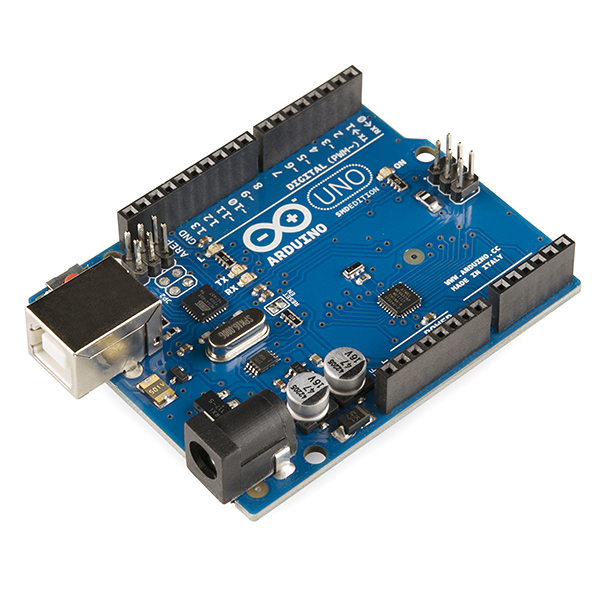
\includegraphics[width=0.5\textwidth]{figures/Arduino_Uno_-_R3.jpg}
\caption{Arduino UNO R3.}
\label{Arduino}
\end{figure}
Figure \ref{Arduino} shows the Arduino we have used.
\begin{table}[H]
\centering
\caption{Specification of Arduino UNO R3}
\begin{tabular}{|l|l|}
\hline
\multicolumn{1}{|c|}{\cellcolor[HTML]{FFFFFF}{\color[HTML]{333333} \textbf{Characteristics}}} & \textbf{Specification} \\ \hline
Chip                                                                                    & ATmega328P             \\ \hline
Operating voltage                                                                       & 5V                     \\ \hline
Digital i/o pin                                                                         & 14                     \\ \hline
Analogue i/o pin                                                                        & 6                      \\ \hline
DC current for each pin                                                                 & 20mA                   \\ \hline
Flash memory                                                                            & 32KB                   \\ \hline
EEPROM                                                                                  & 1KB                    \\ \hline
Dimension                                                                               & 68.6mm*53.4mm          \\ \hline
Weight                                                                                  & 25g                    \\ \hline
\end{tabular}
\end{table}





\subsection{GSM Module}
A GSM module is a hardware device that uses mobile GSM technology, which provides a data connection with a remote network. In the view of the cell phone network, the basic requirement for a SIM to identify with that network is the same as ordinary mobile telephones.
\begin{figure}[h]
\centering
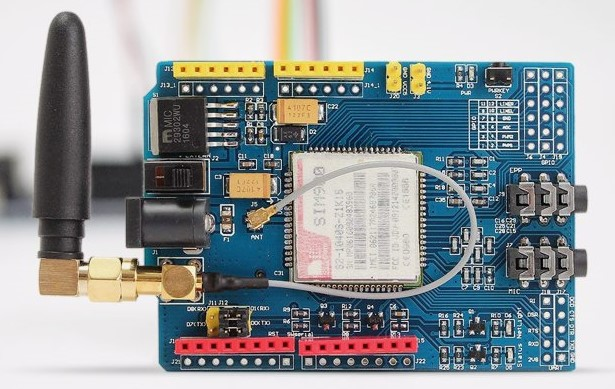
\includegraphics[width=0.5\textwidth]{figures/gsm_module.jpg}
\caption{GSM module.}
\label{GSM}
\end{figure}
Figure \ref{GSM} shows the GSM Module we have used.
\vspace{1cm}


\begin{table}[H]
\centering
\caption{Specification of GSM}
\begin{tabular}{|
>{\columncolor[HTML]{FFFFFF}}c |
>{\columncolor[HTML]{FFFFFF}}c |
>{\columncolor[HTML]{FFFFFF}}c |}
\hline
{\color[HTML]{333333} \textbf{Modes}}                              & {\color[HTML]{333333} \textbf{Frequency}} & {\color[HTML]{333333} \textbf{Current Consumption}} \\ \hline
{\color[HTML]{333333} Power down}                                  & {\color[HTML]{333333} }                   & {\color[HTML]{333333} 60 uA}                        \\ \hline
{\color[HTML]{333333} Sleep mode}                                  & {\color[HTML]{333333} }                   & {\color[HTML]{333333} 1 mA}                         \\ \hline
{\color[HTML]{333333} Stand by}                                    & {\color[HTML]{333333} }                   & {\color[HTML]{333333} 18 mA}                        \\ \hline
\cellcolor[HTML]{FFFFFF}{\color[HTML]{333333} }                       & {\color[HTML]{333333} GSM850}             & {\color[HTML]{333333} 199 mA}                       \\ \cline{2-3} 
\cellcolor[HTML]{FFFFFF}{\color[HTML]{333333} }                       & {\color[HTML]{333333} EGSM900}            & {\color[HTML]{333333} 216 mA}                       \\ \cline{2-3} 
\cellcolor[HTML]{FFFFFF}{\color[HTML]{333333} }                       & {\color[HTML]{333333} DCS1800}            & {\color[HTML]{333333} 146 mA}                       \\ \cline{2-3} 
\multirow{-4}{*}{\cellcolor[HTML]{FFFFFF}{\color[HTML]{333333} Call}} & {\color[HTML]{333333} PCS1900}            & {\color[HTML]{333333} 131 mA}                       \\ \hline
{\color[HTML]{333333} GPRS}                                        & {\color[HTML]{333333} }                   & {\color[HTML]{333333} 453 mA}                       \\ \hline
{\color[HTML]{333333} Transmission burst}                          & {\color[HTML]{333333} }                   & {\color[HTML]{333333} 2 A}                          \\ \hline
\end{tabular}
\end{table}


\subsection{LCD Display}
Liquid crystal display is the word LCD. It is a type of electric display module used in a wide range of applications such as cell phones, calculators, computers, TV sets and other devices. Mainly for multifaceted light-emitting diodes, these displays are favoured. The key advantages of using these modules are cheap simply programmable, animations and customized characters, unique and even animations etc. are not limited to show. Figure \ref{LCD1} shows the 16*2 LCD we have used.
\begin{figure}[h]
\centering
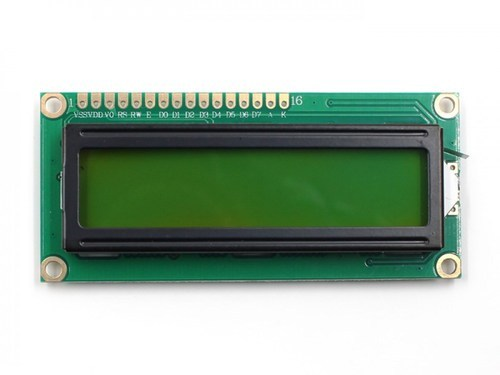
\includegraphics[width=0.5\textwidth]{figures/lcd display.jpg}
\caption{LCD display.}
\label{LCD1}
\end{figure}


\begin{table}[h]
\centering
\caption{Specification of 16*2 LCD}
\begin{tabular}{|l|l|}
\hline
\multicolumn{1}{|c|}{\cellcolor[HTML]{FFFFFF}{\color[HTML]{333333} \textbf{Characteristics}}} & \textbf{Specification} \\ \hline
Operating voltage                                                                       & 4.7V-5.3V              \\ \hline
Power consumption                                                                       & 1mA                    \\ \hline
Cell                                                                                    & 16*2                   \\ \hline
\end{tabular}
\end{table}
\pagebreak

\subsection{Flow Sensor}
The water flow sensor consists of a nickel, a hall-effect sensor and a rotor for the water. When water flows through the rotor, the rotor rolls, with a different flow rate, the speed varies. The more water flows the rolling speed of the rotor becomes high and generates more electricity. Calculating this voltage of the electricity the flowing rate of water is found.
\begin{figure}[h]
\centering
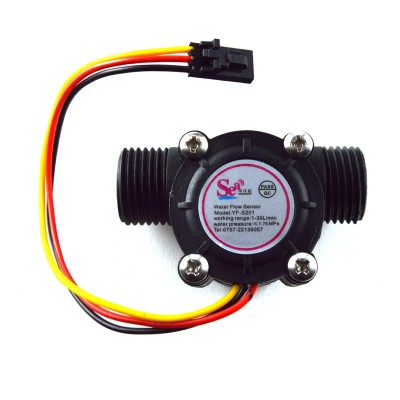
\includegraphics[width=0.5\textwidth]{figures/flow_sensor.jpg}
\caption{Flow sensor.}
\label{Flow1}
\end{figure}
Figure \ref{Flow1} shows the water Flow sensor we have used.

\begin{table}[h]
\centering
\caption{Specification of flow sensor}
\begin{tabular}{|l|l|}
\hline
\multicolumn{1}{|c|}{\cellcolor[HTML]{FFFFFF}{\color[HTML]{333333} \textbf{Characteristics}}} & \textbf{Specification} \\ \hline
Operating voltage                                                                       & 5V                     \\ \hline
Power consumption                                                                       & 15mA                   \\ \hline
Flow rate                                                                               & 1-30L/min              \\ \hline
Operating temperature                                                                   & \textless{}80C         \\ \hline
Liquide temperature                                                                     & \textless{}120C        \\ \hline
Liquid pressure                                                                         & \textless{}2.0MPa      \\ \hline
\end{tabular}
\end{table}

\subsection{pH Sensor}
The acidity or alkalinity of the water is measured with a pH sensor of a value between 0 and 14. The water is becoming more acidic when the pH value falls below 7. Any number higher than seven is more alkaline. In order to calculate water quality, each type of pH sensor works differently.
\begin{figure}[h]
\centering
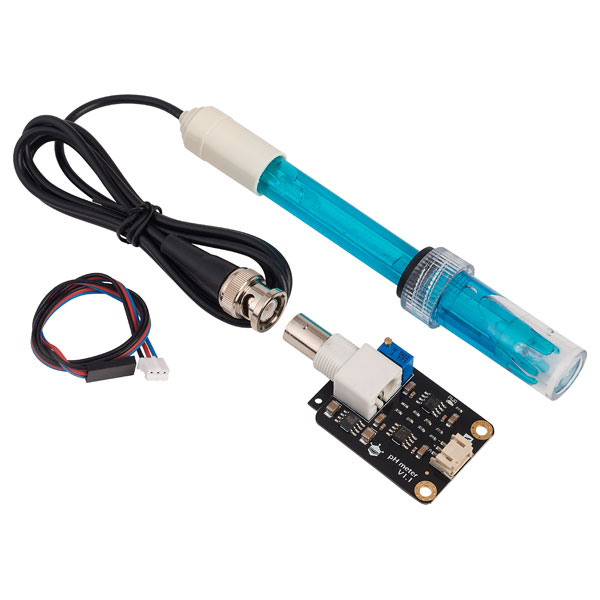
\includegraphics[width=0.5\textwidth]{figures/ph_sensor.jpg}
\caption{pH sensor.}
\label{pH1}
\end{figure}
Figure \ref{pH1} shows the pH sensor we have used.

\begin{table}[H]
\centering
\caption{Specification of pH sensor}
\begin{tabular}{|l|l|}
\hline
\multicolumn{1}{|c|}{\cellcolor[HTML]{FFFFFF}{\color[HTML]{333333} \textbf{Characteristics}}} & \textbf{Specification} \\ \hline
Operating voltage                                                                       & 3.3V-5V                \\ \hline
Range                                                                                   & 0-14pH                 \\ \hline
Probe                                                                                   & BNC                    \\ \hline
Operating temperature                                                                   & \textless{}80C         \\ \hline
Response time                                                                           & \textless{}1min        \\ \hline
\end{tabular}
\end{table}

\subsection{Sonar sensor}
The 4-pin, ground, VCC, trig and echo HC-SR04 Ultrasound Module. Ultrasound sonar sensor has two different sensors one is for transmitting Ultrasound and the other is for receiving the echoed ultrasound. by calculating the time between transmitting and receiving ultrasound the distance is measured. The module pins of ground and VCC have to be wired respectively to the ground with five volt pins on the Arduino board and to any digital I/O pin on the Arduino board with trig and echo pins.
\begin{figure}[h]
\centering
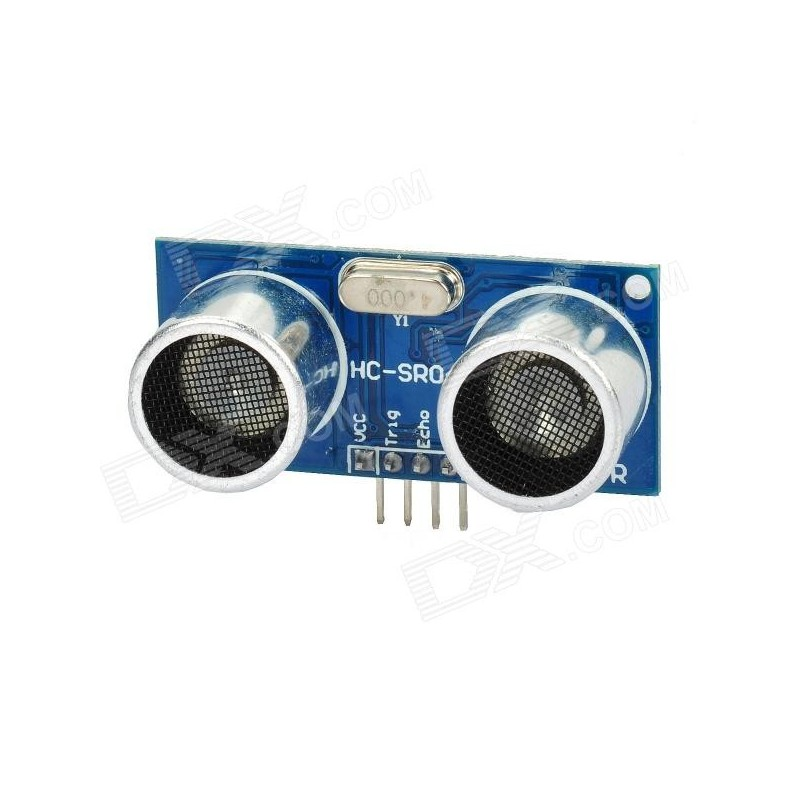
\includegraphics[width=0.5\textwidth]{figures/sonar_sensor.jpg}
\caption{Sonar Sensor.}
\label{Sonar1}
\end{figure}
Figure \ref{Sonar1} shows the Ultrasonic sensor we have used.

\begin{table}[H]
\centering
\caption{Specification of sonar sensor}
\begin{tabular}{|l|l|}
\hline
\multicolumn{1}{|c|}{\cellcolor[HTML]{FFFFFF}{\color[HTML]{333333} \textbf{Characteristics}}} & \textbf{Specification} \\ \hline
Operating voltage                                                                       & 3.5V-5V                \\ \hline
Operating current                                                                       & 2mA                    \\ \hline
Range                                                                                   & 2-400cm                \\ \hline
Angle                                                                                   & \textless{}20          \\ \hline
Accuracy                                                                                & 3mm                    \\ \hline
\end{tabular}
\end{table}

\subsection{Temperature Sensor}
DS18B20 is a Dallas Semiconductor Corp. One wire interface temperature sensor. For a two-way communication with a microcontroller, the special one wire interface needs just one digital pin. The sensor normally comes in two different shapes. One in TO-92 looks like a common transistor exactly. Another one in waterproof form, which can be more useful when measuring anything far, below or below the floor.
The temperature sensor DS18B20 is very accurate and does not require external components. With a precision of ±0.5°C, temperatures range between -55°C and +125°C.

\begin{figure}[h]
\centering
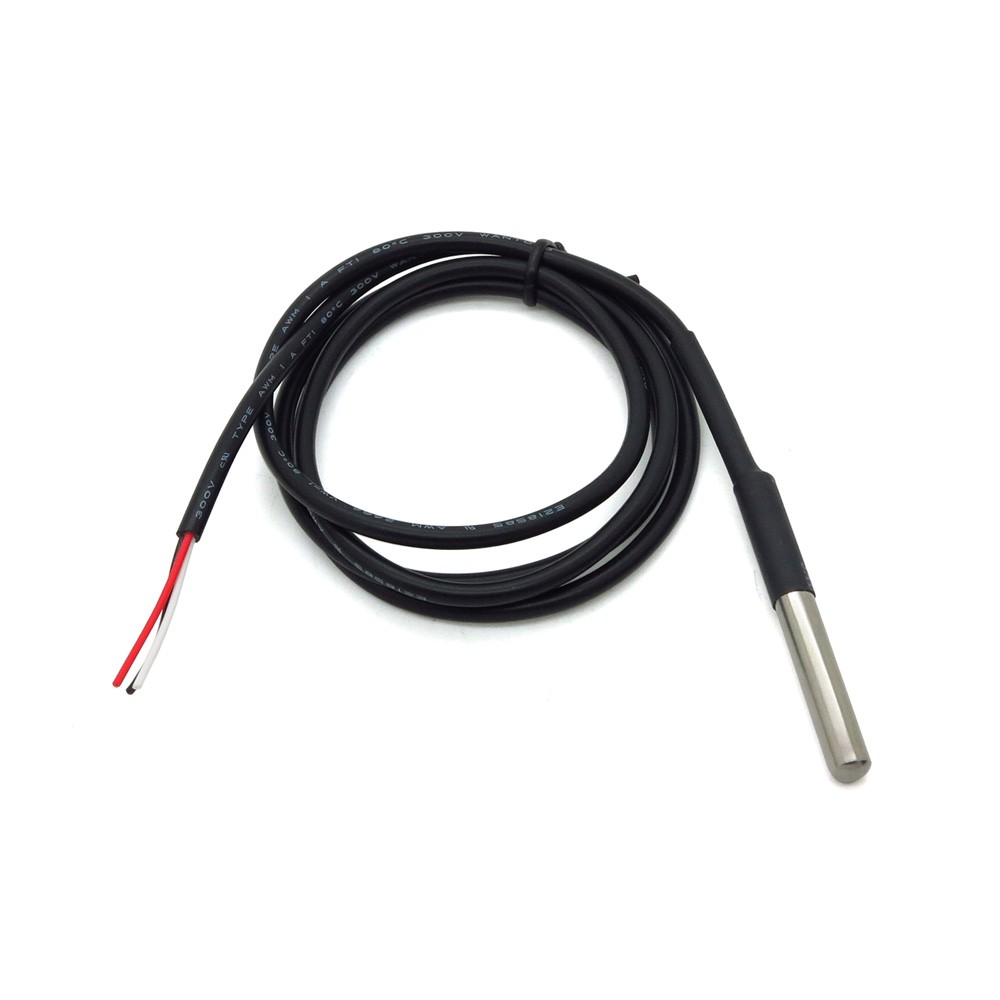
\includegraphics[width=0.5\textwidth]{figures/temperature_sensor.jpg}
\caption{Temperature sensor.}
\label{Temp1}
\end{figure}
Figure \ref{Temp1} shows the water temperature sensor we have used.


\begin{table}[H]
\centering
\caption{Specification of waterproof temperature sensor}
\begin{tabular}{|l|l|}
\hline
\multicolumn{1}{|c|}{\cellcolor[HTML]{FFFFFF}{\color[HTML]{333333} \textbf{Characteristics}}} & \textbf{Specification} \\ \hline
Operating voltage                                                                       & 3.0V-5V                \\ \hline
Operating current                                                                       & 30mA                   \\ \hline
Range                                                                                   & -55C-125C              \\ \hline
Response time                                                                            & \textless{}750ms       \\ \hline
Accuracy                                                                                & 0.5C                   \\ \hline
\end{tabular}
\end{table}

\subsection{Turbidity Sensor}
By testing turbidity levels and opaqueness, the gravitational Arduino turbidity sensor detects water quality. It uses infrared light to measure the transmission of light and dispersion rates to detect suspended particles in water, which varies with the total suspended solids (TSS) in water. The liquid turbidity level increases as the TSS increases. Sensors for sediment transport and laboratories tests are used for measuring water quality in the streams and rivers, wastewater and effluent measurements, inspection devices for sediment sedimentation pools.
\begin{figure}[h]
\centering
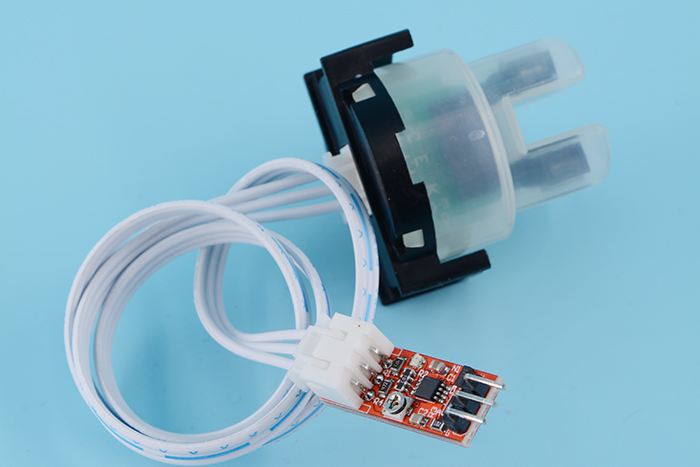
\includegraphics[width=0.5\textwidth]{figures/turbidity_sensor.jpg}
\caption{Turbidity sensor.}
\label{Turbidity1}
\end{figure}
Figure \ref{Turbidity1} shows the Turbidity sensor we have used.

\begin{table}[H]
\centering
\caption{Specification of turbidity sensor}
\begin{tabular}{|l|l|}
\hline
\multicolumn{1}{|c|}{\cellcolor[HTML]{FFFFFF}{\color[HTML]{333333} \textbf{Characteristics}}} & \textbf{Specification} \\ \hline
Operating voltage                                                                       & 5V                     \\ \hline
Operating current                                                                       & 40mA                   \\ \hline
Range                                                                                   & -55C-125C              \\ \hline
Response time                                                                            & \textless{}500ms       \\ \hline
Weight                                                                                  & 30g                    \\ \hline
\end{tabular}
\end{table}

\subsection{GPS Module}
GPS modules contain small antennas and processors which receive direct data from satellites via specific RF frequencies. From there, along with other data bits, it is going to receive timelines from each visible satellite. If an antenna of the module can spot four or more satellites, its location and time can be accurately calculated.
\begin{figure}[h]
\centering
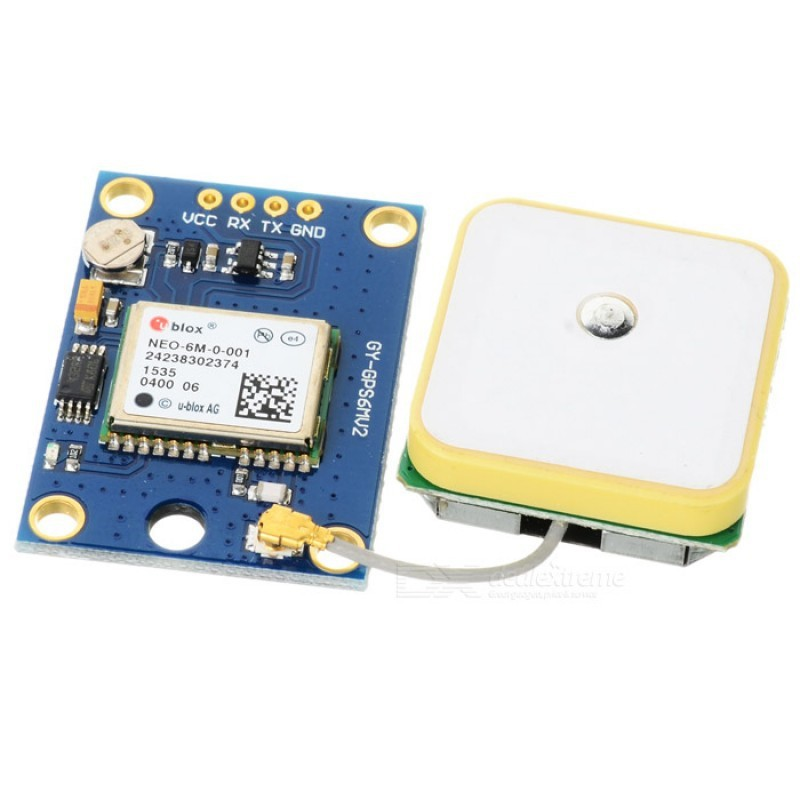
\includegraphics[width=0.5\textwidth]{figures/neo_6m_gps_module.jpg}
\caption{GPS module.}
\label{GPS1}
\end{figure}
Figure \ref{GPS1} shows the GPS sensor we have used to get Location.

\begin{table}[H]
\centering
\caption{Specification of Neo 6m GPS module}
\begin{tabular}{|l|l|}
\hline
\multicolumn{1}{|c|}{\cellcolor[HTML]{FFFFFF}{\color[HTML]{333333} \textbf{Characteristics}}} & \textbf{Specification} \\ \hline
Operating voltage                                                                       & 3.3-6V                 \\ \hline
Baud rate                                                                               & 4800-115200            \\ \hline
Channel                                                                                 & 50                     \\ \hline
Response time                                                                            & \textless{}1s          \\ \hline
Accuracy                                                                                & 2m                     \\ \hline
Update rate                                                                             & 5Hz                    \\ \hline
\end{tabular}
\end{table}

\subsection{Non Return Valve}
A non-return valve can only allow the liquid medium to flow in one direction and is installed to ensure that the medium flows in the correct direction through a pipe, where otherwise the pressure conditions can cause opening the gate for reverse flow.
\begin{figure}[h]
\centering
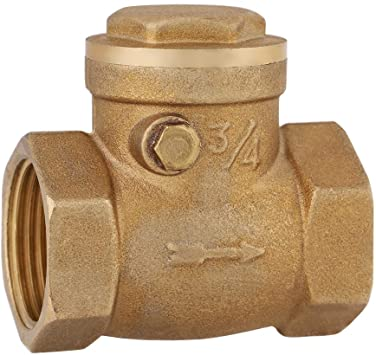
\includegraphics[width=0.5\textwidth]{figures/non_return_valve.jpg}
\caption{Non return valve.}
\label{Valve1}
\end{figure}
Figure \ref{Valve1} shows the non return water gate we have used for flushing water.

\begin{table}[H]
\centering
\caption{Specification of non return valve}
\begin{tabular}{|l|l|}
\hline
\multicolumn{1}{|c|}{\cellcolor[HTML]{FFFFFF}{\color[HTML]{333333} \textbf{Characteristics}}} & \textbf{Specification} \\ \hline
Size                                                                                    & 80mm                   \\ \hline
Material                                                                                & Brass                  \\ \hline
Media                                                                                   & Air, water, gas        \\ \hline
\end{tabular}
\end{table}

\subsection{Servo Motor}
A Servo Motor is a small output shaft unit. By giving the servo a coded signal, this shaft can be located in particular angular positions. The servo retains the angular location of the shaft as long as the coded signal remains on the input side. The angular direction of the shaft changes if the coded signal changes. Servos are used for positioning control surfaces such as elevators and rudders in practice in radio-controlled aircraft. They are also used in boat, motorcycles, marionettes, and of course, robots that are radio powered.
\begin{figure}[h]
\centering
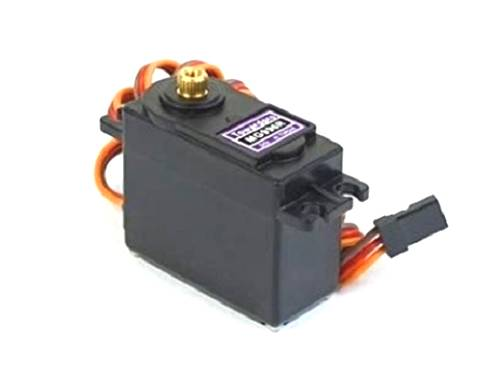
\includegraphics[width=0.5\textwidth]{figures/MG996R-Servo-Motor.jpg}
\caption{Servo motor.}
\label{Servo1}
\end{figure}
Figure \ref{Servo1} shows the Servo motor we have used for opening and closing water gate.

\begin{table}[H]
\centering
\caption{Specification of servo motor}
\begin{tabular}{|l|l|}
\hline
\multicolumn{1}{|c|}{\cellcolor[HTML]{FFFFFF}{\color[HTML]{333333} \textbf{Characteristics}}} & \textbf{Specification} \\ \hline
Operating voltage                                                                       & 4.8-7.2V               \\ \hline
Speed                                                                                   & 0.16s/60deg            \\ \hline
Torque                                                                                  & 12kg/cm                \\ \hline
Operating temperature                                                                   & -30C-60C               \\ \hline
Gear type                                                                               & metal                  \\ \hline
Range                                                                                   & 0-180deg               \\ \hline
\end{tabular}
\end{table}

\subsection{NodeMCU  ESP8266}
ESP8266 is a wifi module that is low powered devices. It can operate in a 2.4GHz network by which it can easily be connected to any wifi network. It has a library for being connected to a remote server to send and retrieve data. It is very easy to use and to combine with another Arduino. The specifications are given below. 
\begin{figure}[h]
\centering
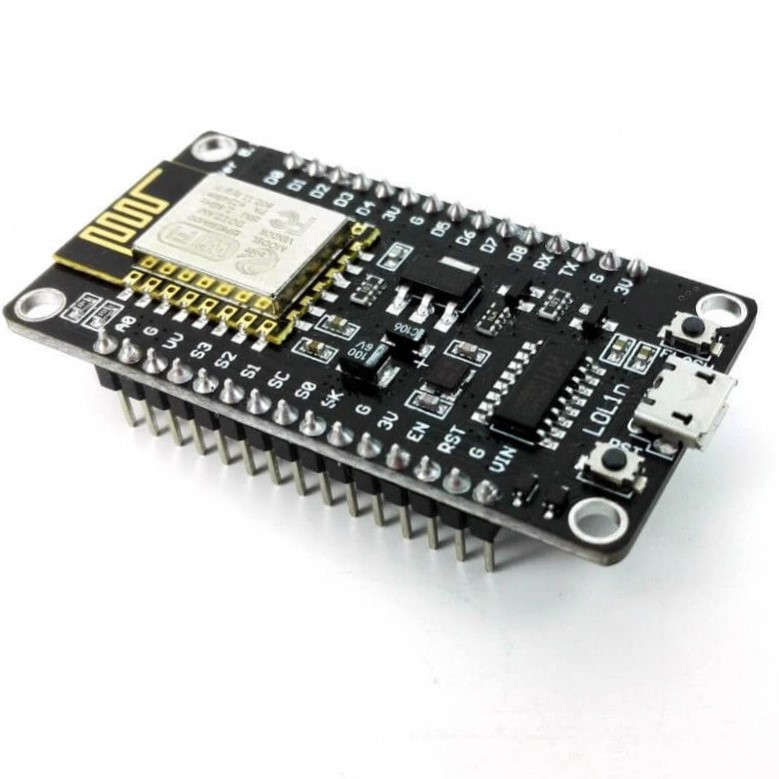
\includegraphics[width=0.5\textwidth]{figures/wifi_module.jpg}
\caption{Wifi module.}
\label{NodeMCU1}
\end{figure}
Figure \ref{NodeMCU1} shows the ESP8266 NodeMCU we have used for internet connection.

\begin{table}[H]
\centering
\caption{Specification of ESP8266 wifi module}
\begin{tabular}{|l|l|}
\hline
\multicolumn{1}{|c|}{\cellcolor[HTML]{FFFFFF}{\color[HTML]{333333} \textbf{Characteristics}}} & \textbf{Specification} \\ \hline
Chip                                                                                    & 32-bit RISC CPU        \\ \hline
Operating voltage                                                                       & 3.3V-5V                \\ \hline
GPIO pin                                                                                & 16                     \\ \hline
Analogue i/o pin                                                                        & 1                      \\ \hline
DC current for each pin                                                                 & 20mA                   \\ \hline
Flash memory                                                                            & 64KB                   \\ \hline
Network                                                                                 & 2.4GHz(802.11 b/g/n)   \\ \hline
\end{tabular}
\end{table}

\subsection{Buzzer}
It is a light weight frequency making device made of piezoelectric crystal
\begin{figure}[h]
\centering
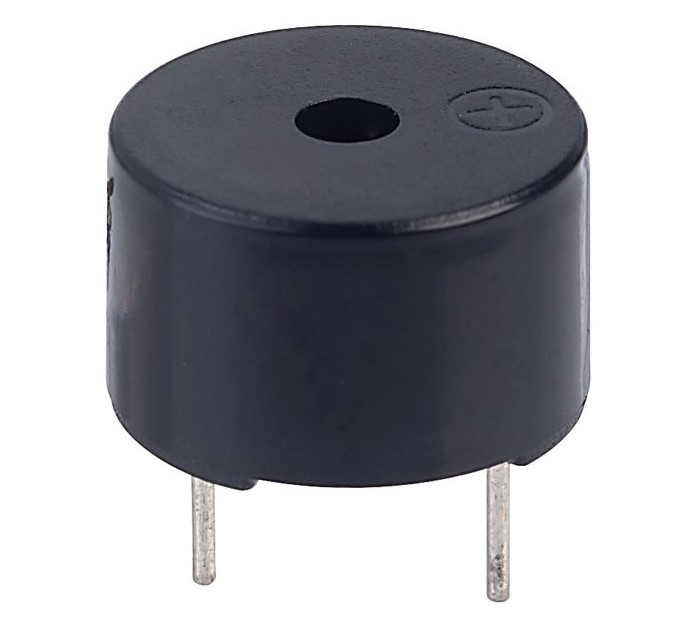
\includegraphics[width=0.5\textwidth]{figures/buzzer.jpg}
\caption{Buzzer.}
\label{Buzzer1}
\end{figure}
Figure \ref{Buzzer1} shows the buzzer we have used for making early alarm.

\begin{table}[H]
\centering
\caption{Specification of buzzer}
\begin{tabular}{|l|l|}
\hline
\multicolumn{1}{|c|}{\cellcolor[HTML]{FFFFFF}{\color[HTML]{333333} \textbf{Characteristics}}} & \textbf{Specification} \\ \hline
Operating voltage                                                                             & 3.3V-6V                \\ \hline
Current                                                                                       & \textless{}25mA        \\ \hline
Frequency                                                                                     & 2300Hz                 \\ \hline
Operating temperature                                                                         & -20C-60C               \\ \hline
Weight                                                                                        & 2.5g                   \\ \hline
\end{tabular}
\end{table}
\subsection{Brush}
A Brush made of nylon is used to clean the water tank.

\begin{figure}[h]
    \centering
    \begin{subfigure}[b]{0.3\textwidth}
        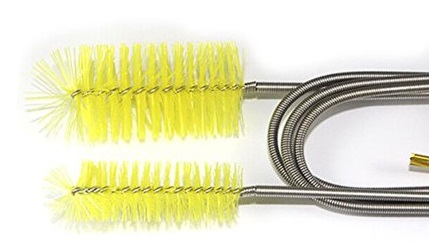
\includegraphics[width=\textwidth]{figures/brush.jpeg}
\caption{Brush.}
\label{Brush1}
    \end{subfigure}
     
        \begin{subfigure}[b]{0.3\textwidth}
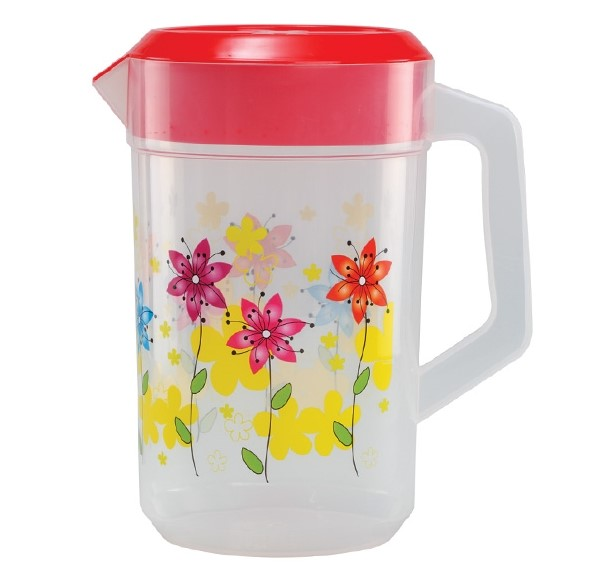
\includegraphics[width=\textwidth]{figures/jug.jpeg}
\caption{Jug.}
\label{Jug1}
    \end{subfigure}
       \caption{Brush and Jug}
     \label{BrushANdJug}
    \end{figure}
Figure \ref{Brush1} shows the Cleaning brush we have used for cleaning the tank.
\subsection{Jug as Water Tank}
A Jug is used as a water tank 
Figure \ref{Jug1} shows the Jug we have used as water tank.

\begin{table}[h]
\centering
\caption{Specification of water jug}
\begin{tabular}{|l|l|}
\hline
\multicolumn{1}{|c|}{\cellcolor[HTML]{FFFFFF}{\color[HTML]{333333} \textbf{Characteristics}}} & \textbf{Specification} \\ \hline
Material                                                                                      & polypropylene          \\ \hline
Colour                                                                                         & transparent            \\ \hline
Net weight                                                                                    & 3.5L                   \\ \hline
Dimension                                                                                     & 22cm*16cm*25.5cm       \\ \hline
\end{tabular}
\end{table}

\subsection{Optocoupler}
An optocoupler is a switching device that can switch another device without triggering electrically. It makes two devices optically isolated.

\begin{figure}[h]
\centering
\subfloat[Optocoupler device]{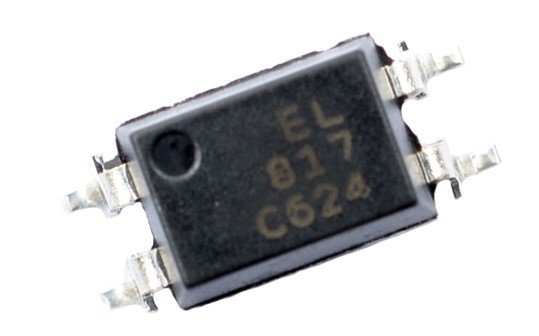
\includegraphics[width = 0.4\textwidth]{figures/optocupler.jpg}} 
\hspace{1in}
\subfloat[Schematic diagram]{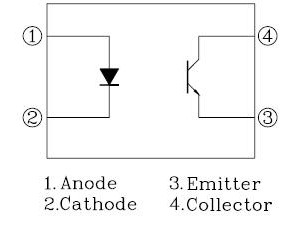
\includegraphics[width = 0.35\textwidth]{figures/optocupler1.jpg}}

\caption{Optocoupler}
\label{Optocupler1}
\end{figure}
Figure \ref{Optocupler1} shows the Optocoupler we have used.

\begin{table}[H]
\centering
\caption{Specification of optocoupler}
\begin{tabular}{|l|l|}
\hline
\multicolumn{1}{|c|}{\cellcolor[HTML]{FFFFFF}{\color[HTML]{333333} \textbf{Characteristics}}} & \textbf{Specification} \\ \hline
Current transfer ratio                                                                        & 600\%                  \\ \hline
Voltage                                                                                       & 5V                     \\ \hline
Current                                                                                       & 5mA                    \\ \hline
Temperature                                                                                   & +110C                  \\ \hline
Type                                                                                          & Switch                 \\ \hline
\end{tabular}
\end{table}

\subsection{Other Equipment}
Other passive equipment like a breadboard, adapter, jumper wire, scotch tape, the gum is used. A breadboard is a kind of board that is used to connect components electrically. 5V Adapter is used for the power source. It converts high voltage to low voltage. Jumper wire used to drive electric.
\begin{figure}[h]
\centering
\subfloat[Breadboard]{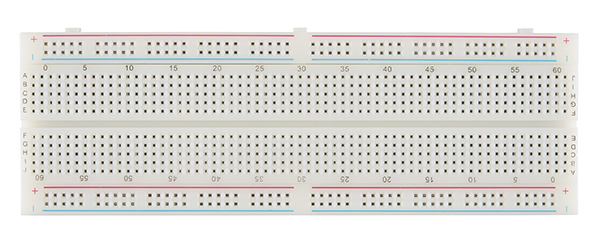
\includegraphics[width = 0.3\textwidth]{figures/breadboard.jpg}} 
\hspace{1cm}
\subfloat[Jumper wire]{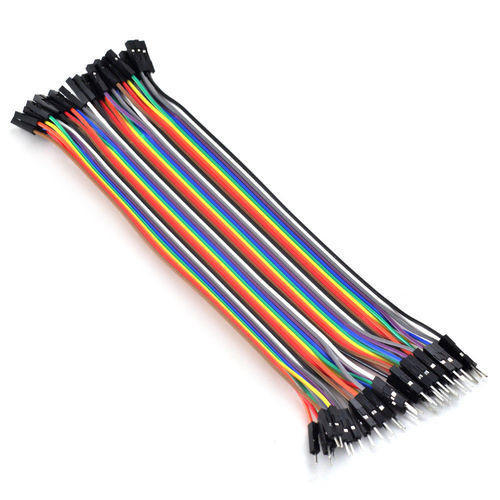
\includegraphics[width = 0.3\textwidth]{figures/jumperwire.jpg}}
\hspace{1cm}
\subfloat[Adapter]{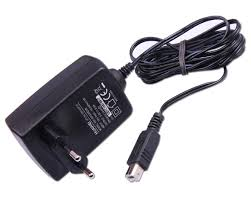
\includegraphics[width = 0.3\textwidth]{figures/adapter.jpg}}

\caption{Other components}
\label{Other1}
\end{figure}
Figure \ref{Other1} shows other passive components we have used.


\section{Software Specification}
In this section we will discuss about some software that we have used in our system.
\subsection{Arduino IDE}
This platform is for writing code for Arduino board. It is a C language base IDE. It has the own compiler and library installed on different Arduino board. Using this IDE code editing, debugging and loading can be done in Arduino board. It has a serial monitor by which any real time value can be seen. It is very easy to learn and use.
\begin{figure}[h]
\centering

\includegraphics[width=0.5\textwidth]{figures/arduino_ide.jpg}
\caption{Arduino IDE Icon}
\label{Arduino1}
\end{figure}
Figure \ref{Arduino1} shows Arduino IDE  we have used.
\pagebreak
\subsection{Android Studio}
This platform is made by IntelliJ for writing code for android device. It is a java and extensive markup language (XML) language base IDE. it has its own compiler for android device. Many libraries are previously installed for a different version of the Android operating system. From this platform, code can be edited, dubbed and exported into APK software.
\begin{figure}[h]
\centering

\includegraphics[width=0.5\textwidth]{figures/android_studio.png}
\caption{Android studio}
\label{Android1}
\end{figure}
Figure \ref{Android1} shows Android IDE  we have used.

\subsection{Operating System}
We used windows 10 home as the operating system of our device. This operating system is very user friendly as it is graphically rich.
\begin{figure}[h]
\centering
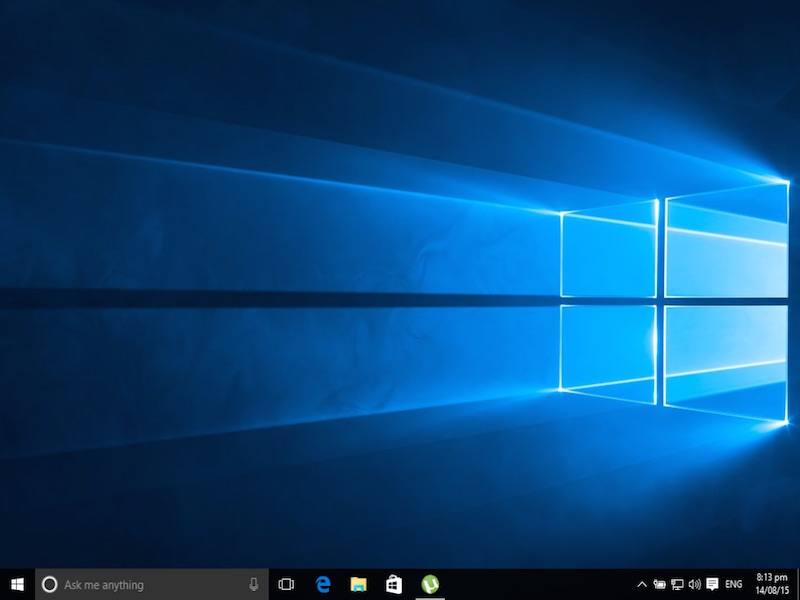
\includegraphics[width=0.5\textwidth]{figures/windows_10.jpg}
\caption{Windows 10}
\label{OS1}
\end{figure}
Figure \ref{OS1} shows Operating System  we have used.

\pagebreak
\subsection{Firebase}
We used the firebase realtime database as the cloud server of our system's database. This platform is made by google. It is free, fast and easy to use. It has SDK for android code and also API for Arduino code so integration is easy.
\begin{figure}[h]
\centering
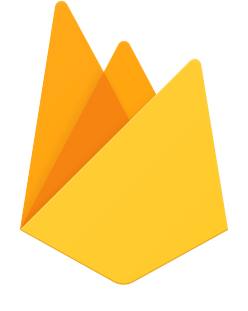
\includegraphics[width=0.35\textwidth]{figures/firebase.png}
\caption{Firebase}
\label{Firebase1}
\end{figure}
Figure \ref{Firebase1} shows Firebase  we have used as realtime database.

% \subsection{Android application}
% We developed an android application that is very easy to use. It can retrieve the data stored on the firebase real-time database.
% \begin{figure}[H]
% \centering
% 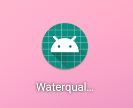
\includegraphics[width=0.4\textwidth]{figures/application_icon.JPG}
% \caption{Application Icon}
% \label{sample}
% \end{figure}


\subsection{Implementation Challenges}
\begin{itemize}
\item Making this system watertight
\item Insulating electronics from water
\item Data Storage Challenge.
\item Connectivity and Power Management IoT Challenges.
\item Data Security Issues.
\item Authentication and Identification Issues in IoT.
\item Managing all components in this lockdown situation
\item Making this system simpler thus it works perfectly and complexity to be minimum
\end{itemize}

\section{Conclusion}
A systematic analysis of the literature is discussed in this chapter. This topic was conveniently divided into key sections of the monitoring and control segment for water quality. We explained various hardware and software equipment here. The following chapter provides vast explanations of the proposed water quality monitoring and controlling system's methodology.
